\section{Results} \label{sec:results}

We employ the optimization described above (see \equref{eq:opt}) in an interactive freeform editing system. The input to our system is the flat domain boundary and the curves of the crease pattern, represented by polylines. These can be easily generated from any standard vector graphics format by sampling the smooth curves therein. Our system computes an arrangement of the input curves using CGAL's arrangement model \cite{cgal,cgal_arr1,cgal_arr2} and solves the symmetric indefinite  linear systems as required by the optimization (\equref{eq:linear_system}) using Pardiso \cite{PARDISO1,PARDISO2,PARDISO3}. Our editing system supports setting point handle positional constraints, as can be seen in Figures \ref{fig:teaser}, \ref{fig:multiple_crease_patterns}, and the second and last model from the left in \figref{fig:folded_and_not_folded}. We also support  constraining a crease curve by specifying its curvature and torsion in a curve constrained flow,  see Figures~\ref{fig:folded_and_not_folded} and \ref{fig:MV_bias_modeling}, as well as prescribing a sparse set of dihedral angles along crease points, see \figref{fig:dihedral_editing}. 

\figref{fig:MV_bias_modeling} is the only case where we supply a mountain/valley assignment as input, while \figref{fig:dihedral_editing} display the only models designed by constraining dihedral angles. The curve constrained positional constraints, as well as the dihedral angles are interpolated for improved quality (see \figref{fig:homotopy_curve}). To maintain interactive frame rates in handle based editing tasks, we run a fixed number of SQP iterations per frame, which we set to 5. Our system is able to handle realtime interaction of meshes with around 2000 vertices. The two concentric circles fold at \figref{fig:teaser} originates from a mesh with about $5500$ vertices. They were designed by simply penalizing the distance of a single pair of vertices while interpolating that penalty weight, and their final forms was reached in about 30 seconds. We refer the reader to our supplementary video for further results, including interactive editing examples. 

\begin{figure} [h]
	\centering
	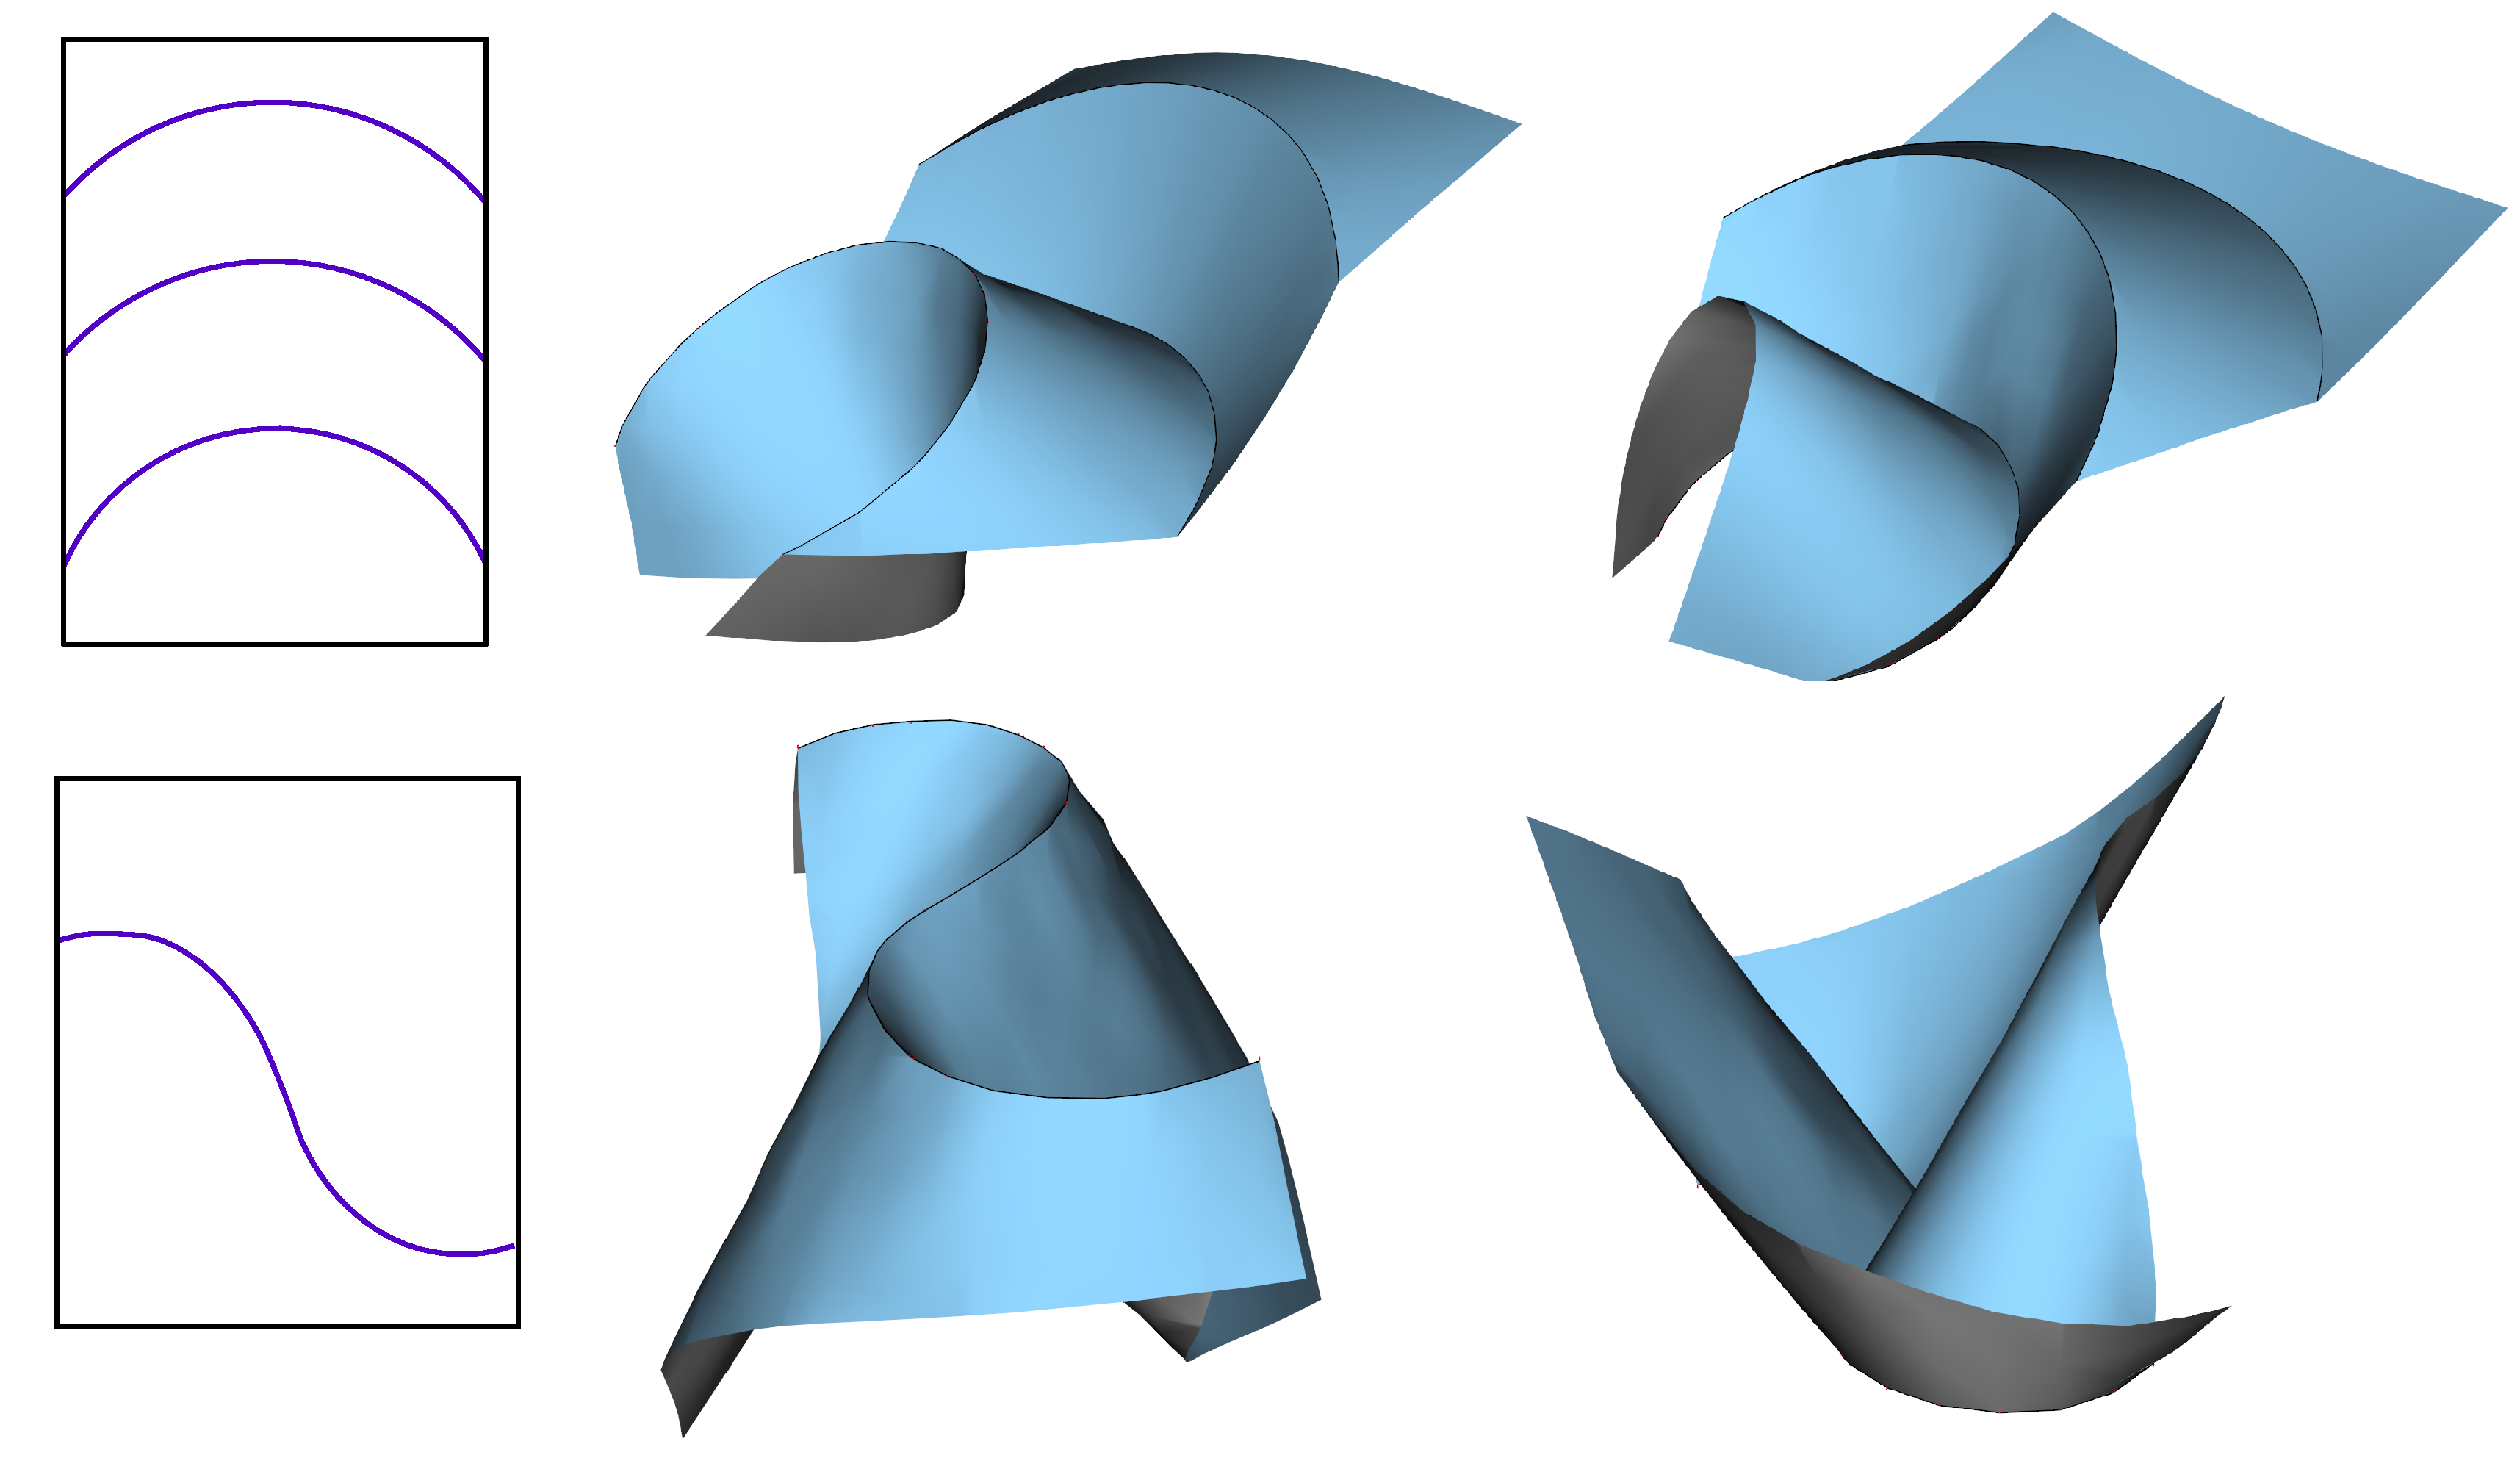
\includegraphics[width=\linewidth]{figures/MV_bias_modeling}
	\caption{Using the optional mountain/valley assignment input (\secref{sec:MV_assignments}) on a single crease curve. Each crease pattern is deformed with the same positional constraints, induced by a curve constrained flow, but with a different mountain/valley assignment along one crease, enforced by \equref{eq:mountain_valley}. In the banana shaped model (bottom row), the rest of the mountain/valley assignments are then uniquely determined.}
	\label{fig:MV_bias_modeling}
\end{figure}

\begin{figure} [h]
	\centering
	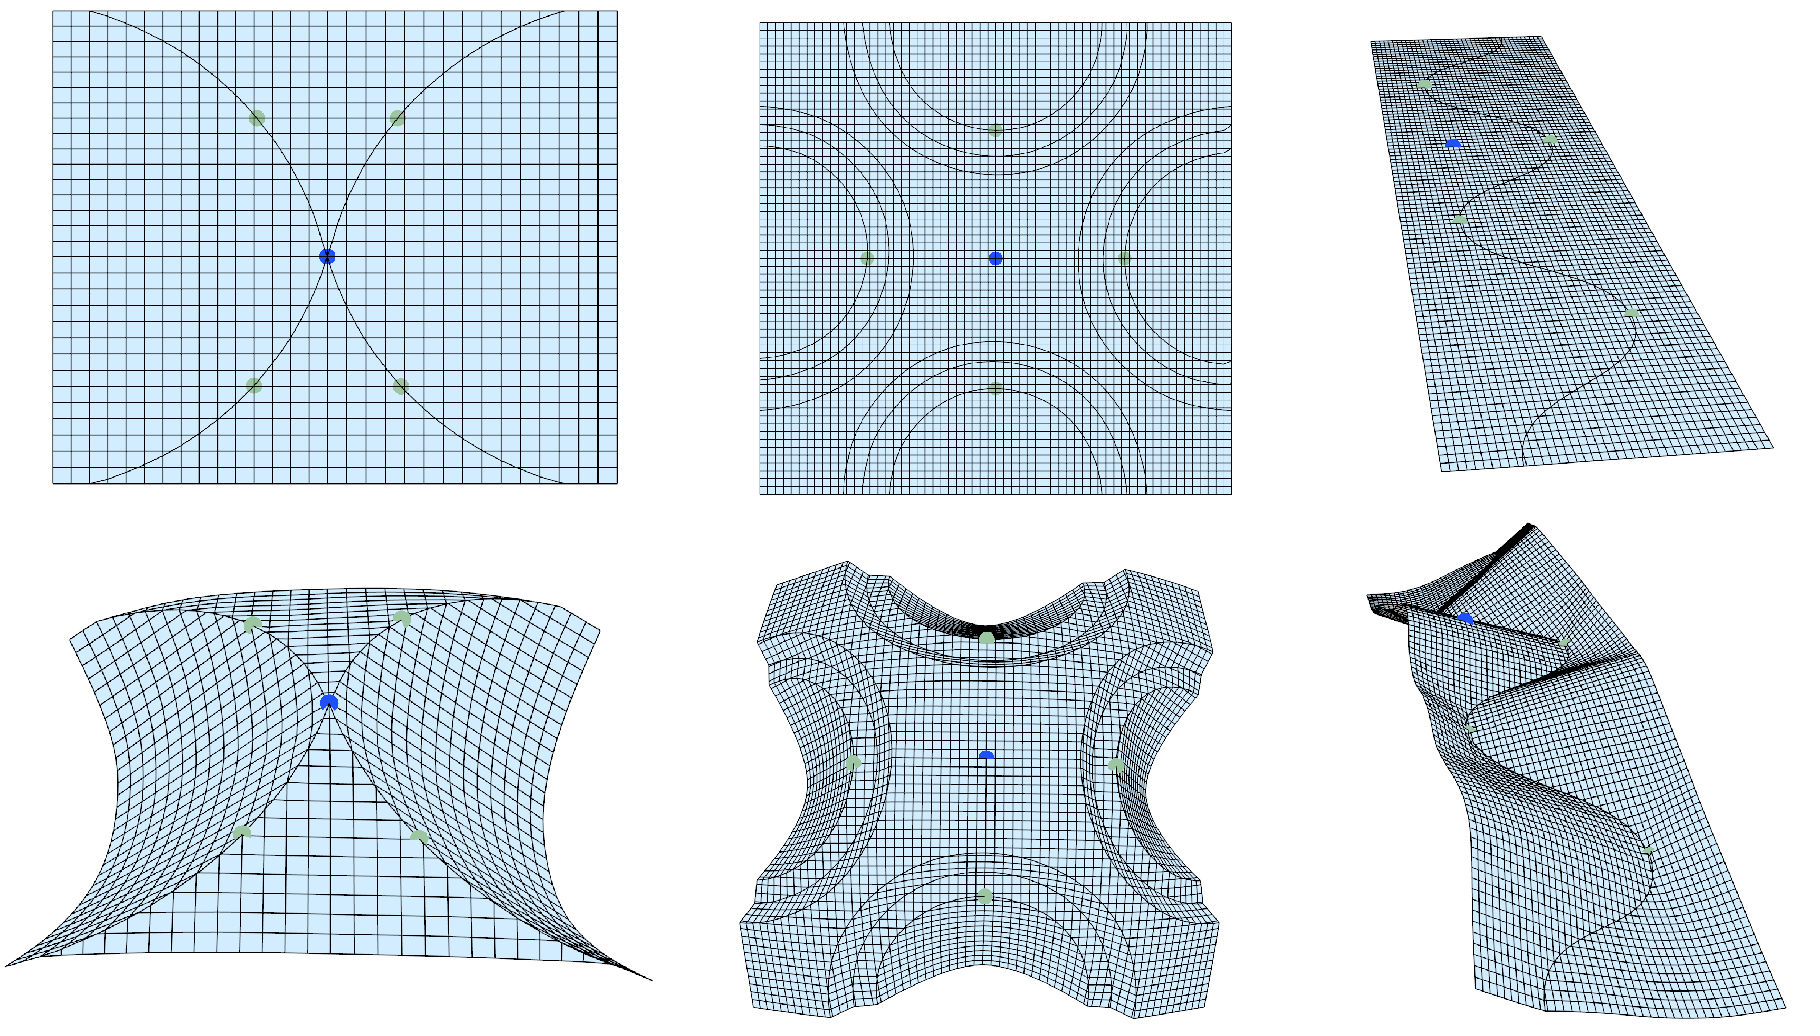
\includegraphics[width=\linewidth]{figures/dihedral_editing}
	\caption{Using the optional folding angle constraints (\secref{sec:folding_angle}) on a spare set of crease points. These examples are deformed by constraining the folding angle of a set of points (in green), without specifying their folding orientation, and by setting a single positional constraint (in blue).}
	\label{fig:dihedral_editing}
\end{figure}